\section*{Problem 7}
We use the code from the book as a guide and flesh out the following script

\inputminted{python}{P7script.py}

\pagebreak

The output images are as follows
\begin{figure*}[h]
    \centering
    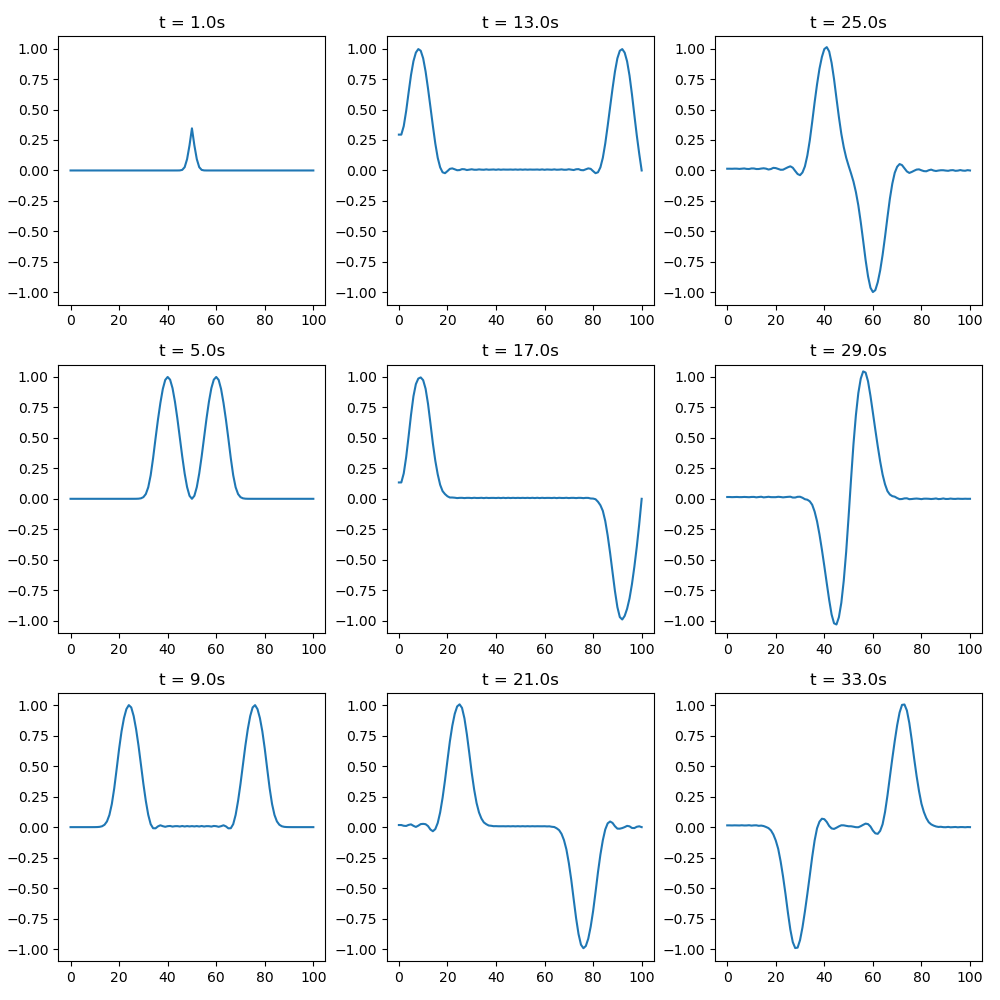
\includegraphics[scale=0.55]{figures/P7output}
\end{figure*}

We see that The pulse hitting the stress free boundary is reflected as is but the pulse hitting the fixed boundary has its displacement mirrored as it is reflected back. When the pulses meet they pass through each other.